% Options for packages loaded elsewhere
\PassOptionsToPackage{unicode}{hyperref}
\PassOptionsToPackage{hyphens}{url}
\PassOptionsToPackage{dvipsnames,svgnames,x11names}{xcolor}
%
\documentclass[
  letterpaper,
]{ut-thesis}

\usepackage{amsmath,amssymb}
\usepackage{iftex}
\ifPDFTeX
  \usepackage[T1]{fontenc}
  \usepackage[utf8]{inputenc}
  \usepackage{textcomp} % provide euro and other symbols
\else % if luatex or xetex
  \usepackage{unicode-math}
  \defaultfontfeatures{Scale=MatchLowercase}
  \defaultfontfeatures[\rmfamily]{Ligatures=TeX,Scale=1}
\fi
\usepackage{lmodern}
\ifPDFTeX\else  
    % xetex/luatex font selection
\fi
% Use upquote if available, for straight quotes in verbatim environments
\IfFileExists{upquote.sty}{\usepackage{upquote}}{}
\IfFileExists{microtype.sty}{% use microtype if available
  \usepackage[]{microtype}
  \UseMicrotypeSet[protrusion]{basicmath} % disable protrusion for tt fonts
}{}
\makeatletter
\@ifundefined{KOMAClassName}{% if non-KOMA class
  \IfFileExists{parskip.sty}{%
    \usepackage{parskip}
  }{% else
    \setlength{\parindent}{0pt}
    \setlength{\parskip}{6pt plus 2pt minus 1pt}}
}{% if KOMA class
  \KOMAoptions{parskip=half}}
\makeatother
\usepackage{xcolor}
\setlength{\emergencystretch}{3em} % prevent overfull lines
\setcounter{secnumdepth}{5}
% Make \paragraph and \subparagraph free-standing
\makeatletter
\ifx\paragraph\undefined\else
  \let\oldparagraph\paragraph
  \renewcommand{\paragraph}{
    \@ifstar
      \xxxParagraphStar
      \xxxParagraphNoStar
  }
  \newcommand{\xxxParagraphStar}[1]{\oldparagraph*{#1}\mbox{}}
  \newcommand{\xxxParagraphNoStar}[1]{\oldparagraph{#1}\mbox{}}
\fi
\ifx\subparagraph\undefined\else
  \let\oldsubparagraph\subparagraph
  \renewcommand{\subparagraph}{
    \@ifstar
      \xxxSubParagraphStar
      \xxxSubParagraphNoStar
  }
  \newcommand{\xxxSubParagraphStar}[1]{\oldsubparagraph*{#1}\mbox{}}
  \newcommand{\xxxSubParagraphNoStar}[1]{\oldsubparagraph{#1}\mbox{}}
\fi
\makeatother


\providecommand{\tightlist}{%
  \setlength{\itemsep}{0pt}\setlength{\parskip}{0pt}}\usepackage{longtable,booktabs,array}
\usepackage{calc} % for calculating minipage widths
% Correct order of tables after \paragraph or \subparagraph
\usepackage{etoolbox}
\makeatletter
\patchcmd\longtable{\par}{\if@noskipsec\mbox{}\fi\par}{}{}
\makeatother
% Allow footnotes in longtable head/foot
\IfFileExists{footnotehyper.sty}{\usepackage{footnotehyper}}{\usepackage{footnote}}
\makesavenoteenv{longtable}
\usepackage{graphicx}
\makeatletter
\newsavebox\pandoc@box
\newcommand*\pandocbounded[1]{% scales image to fit in text height/width
  \sbox\pandoc@box{#1}%
  \Gscale@div\@tempa{\textheight}{\dimexpr\ht\pandoc@box+\dp\pandoc@box\relax}%
  \Gscale@div\@tempb{\linewidth}{\wd\pandoc@box}%
  \ifdim\@tempb\p@<\@tempa\p@\let\@tempa\@tempb\fi% select the smaller of both
  \ifdim\@tempa\p@<\p@\scalebox{\@tempa}{\usebox\pandoc@box}%
  \else\usebox{\pandoc@box}%
  \fi%
}
% Set default figure placement to htbp
\def\fps@figure{htbp}
\makeatother
% definitions for citeproc citations
\NewDocumentCommand\citeproctext{}{}
\NewDocumentCommand\citeproc{mm}{%
  \begingroup\def\citeproctext{#2}\cite{#1}\endgroup}
\makeatletter
 % allow citations to break across lines
 \let\@cite@ofmt\@firstofone
 % avoid brackets around text for \cite:
 \def\@biblabel#1{}
 \def\@cite#1#2{{#1\if@tempswa , #2\fi}}
\makeatother
\newlength{\cslhangindent}
\setlength{\cslhangindent}{1.5em}
\newlength{\csllabelwidth}
\setlength{\csllabelwidth}{3em}
\newenvironment{CSLReferences}[2] % #1 hanging-indent, #2 entry-spacing
 {\begin{list}{}{%
  \setlength{\itemindent}{0pt}
  \setlength{\leftmargin}{0pt}
  \setlength{\parsep}{0pt}
  % turn on hanging indent if param 1 is 1
  \ifodd #1
   \setlength{\leftmargin}{\cslhangindent}
   \setlength{\itemindent}{-1\cslhangindent}
  \fi
  % set entry spacing
  \setlength{\itemsep}{#2\baselineskip}}}
 {\end{list}}
\usepackage{calc}
\newcommand{\CSLBlock}[1]{\hfill\break\parbox[t]{\linewidth}{\strut\ignorespaces#1\strut}}
\newcommand{\CSLLeftMargin}[1]{\parbox[t]{\csllabelwidth}{\strut#1\strut}}
\newcommand{\CSLRightInline}[1]{\parbox[t]{\linewidth - \csllabelwidth}{\strut#1\strut}}
\newcommand{\CSLIndent}[1]{\hspace{\cslhangindent}#1}

\usepackage{booktabs}
\usepackage{longtable}
\usepackage{array}
\usepackage{multirow}
\usepackage{wrapfig}
\usepackage{float}
\usepackage{colortbl}
\usepackage{pdflscape}
\usepackage{tabu}
\usepackage{threeparttable}
\usepackage{threeparttablex}
\usepackage[normalem]{ulem}
\usepackage{makecell}
\usepackage{xcolor}
\usepackage{tocbibind}
\usepackage{pdfpages}
\usepackage{tocloft}
\makeatletter
\@ifpackageloaded{bookmark}{}{\usepackage{bookmark}}
\makeatother
\makeatletter
\@ifpackageloaded{caption}{}{\usepackage{caption}}
\AtBeginDocument{%
\ifdefined\contentsname
  \renewcommand*\contentsname{Table of contents}
\else
  \newcommand\contentsname{Table of contents}
\fi
\ifdefined\listfigurename
  \renewcommand*\listfigurename{List of Figures}
\else
  \newcommand\listfigurename{List of Figures}
\fi
\ifdefined\listtablename
  \renewcommand*\listtablename{List of Tables}
\else
  \newcommand\listtablename{List of Tables}
\fi
\ifdefined\figurename
  \renewcommand*\figurename{Figure}
\else
  \newcommand\figurename{Figure}
\fi
\ifdefined\tablename
  \renewcommand*\tablename{Table}
\else
  \newcommand\tablename{Table}
\fi
}
\@ifpackageloaded{float}{}{\usepackage{float}}
\floatstyle{ruled}
\@ifundefined{c@chapter}{\newfloat{codelisting}{h}{lop}}{\newfloat{codelisting}{h}{lop}[chapter]}
\floatname{codelisting}{Listing}
\newcommand*\listoflistings{\listof{codelisting}{List of Listings}}
\makeatother
\makeatletter
\usepackage{pdflscape}
\makeatother
\makeatletter
\makeatother
\makeatletter
\@ifpackageloaded{caption}{}{\usepackage{caption}}
\@ifpackageloaded{subcaption}{}{\usepackage{subcaption}}
\makeatother

\usepackage{bookmark}

\IfFileExists{xurl.sty}{\usepackage{xurl}}{} % add URL line breaks if available
\urlstyle{same} % disable monospaced font for URLs
\hypersetup{
  pdftitle={Working UofT Thesis Reproducible Report Template using Quarto},
  pdfauthor={Navi Ram},
  colorlinks=true,
  linkcolor={black},
  filecolor={Maroon},
  citecolor={Blue},
  urlcolor={Blue},
  pdfcreator={LaTeX via pandoc}}


\title{Working UofT Thesis Reproducible Report Template using Quarto}
\author{Navi Ram}
\date{2025-07-24}
\degree{Degree}
\gradyear{2025}
\department{Department Name}
\begin{document}
\maketitle
\pagenumbering{roman}
\setcounter{page}{2}
\begin{abstract}
  \addcontentsline{toc}{chapter}{Abstract}
This template allows users to create reproducible documents in the
required UofT thesis formatting using quarto. This quarto book is
written using YAML, R, markdown, and latex syntax. This approach
supports integration with citation managers (e.g.~Zotero) to manage
bibliography and in-text citations, creates cross-referencable figures,
tables, and document sections, generates tables and figures using R
syntax, dynamically inserts acronyms, and allows integration of text and
code. Future updates will introduce APA formatted word doc output
options as well.
\end{abstract}
\begin{acknowledgements}
    \addcontentsline{toc}{chapter}{Acknowledgements}
This would not be possible without the UofT latex template (ut-thesis)
maintained by jessexknight and the acronymsdown package by rchaput
\end{acknowledgements}

\renewcommand*\contentsname{Table of Contents}
{
\hypersetup{linkcolor=}
\setcounter{tocdepth}{2}
\tableofcontents
}
\newpage
\listoftables
\newpage
\listoffigures
\newpage


\newcommand{\listappendicesname}{List of Appendices}
\newlistof{appendices}{apc}{\listappendicesname}
\newcommand{\appendices}[1]{\addcontentsline{apc}{appendices}{#1}}
\parindent0mm

\listofappendices
\addcontentsline{toc}{chapter}{List of Appendices}

\chapter*{List of Acronyms}\label{acronyms_HEADER_LOA}
\addcontentsline{toc}{chapter}{List of Acronyms}

\markboth{List of Acronyms}{List of Acronyms}

\begin{description}
\tightlist
\item[\phantomsection\label{acronyms_ADHD}{ADHD}]
Attention-Deficit/Hyperactivity Disorder
\item[\phantomsection\label{acronyms_EF}{EF}]
Executive Functions
\item[\phantomsection\label{acronyms_RCT}{RCT}]
Randomized Controlled Trial
\item[\phantomsection\label{acronyms_SSRT}{SSRT}]
Stop Signal Reaction Time
\end{description}

\bookmarksetup{startatroot}

\chapter{Introduction}\label{introduction}

\pagenumbering{arabic}

\section{Background}\label{background}

Neurodevelopmental disorders are persistent and impairing lifelong
conditions resulting from combined genetic and environmental influences
(Faraone et al., 2021).
\hyperref[acronyms_ADHD]{Attention-Deficit/Hyperactivity Disorder
(ADHD)} is a highly heritable (Pettersson et al., 2019)
neurodevelopmental disorder diagnosed in approximately 8\% of children
and youth worldwide (Ayano et al., 2023) and is characterized by
persistent inattention and/or hyperactivity symptoms causing impairment
in multiple settings (American Psychiatric Association, 2022). Both
\hyperref[acronyms_ADHD]{ADHD} and autism are associated with a range of
challenges including difficulties with academic achievement, peer
relationships, and behaviour regulation (French et al., 2024; Posar \&
Visconti, 2019). Interventions for \hyperref[acronyms_ADHD]{ADHD}
include use of stimulant or non-stimulant medications, behavioural
parent training, and environmental accommodations (Faraone et al.,
2021). Although each of these may result in improvements at the group
level, benefits are generally time limited and impairment remains in
many individuals (Faraone et al., 2021).

\section{Aim}\label{aim}

Computerized \hyperref[acronyms_EF]{Executive Functions (EF)} training
programs have shown consistent growth in development and investigation,
with several commercial options currently available. The existing
research on efficacy of these programs is variable and largely shows a
lack of far transfer to untrained skills. Most videogame-based
\hyperref[acronyms_EF]{EF} training programs in neurodevelopmental
disorders have focused on ADHD, with more recent work exploring
applications in autism. However, both disorders are characterized by
high heterogeneity in clinical and \hyperref[acronyms_EF]{EF}
characteristics pointing to potential key factors that may be associated
with variability in response to \hyperref[acronyms_EF]{EF} training.
There has been limited investigation on factors associated with
heterogeneity in responses to treatment, which is essential to
understand what intervention works best for whom. To address gaps in the
research on currently available \hyperref[acronyms_EF]{EF} training
programs, our team co-created Mega Team with youth co-designers with a
focus on accessibility, affordability, and multi-skill training. Overall
results of the main \hyperref[acronyms_RCT]{Randomized Controlled Trial
(RCT)} show near and far transfer in ADHD participants but not in
autistic participants (Cheung et al., in prep). This project will
explore a broad range of baseline predictors to better understand
patterns in individual factors of response to computerized
\hyperref[acronyms_EF]{EF} training in a sample of ADHD and/or autism
children.

\textbf{Research Question:} Do demographic (age and gender), clinical
(use of stimulant medication, ADHD symptoms, autism traits),
\hyperref[acronyms_EF]{EF} (response inhibition, working memory baseline
performance, and EF-related impairment), and training (time on task)
factors predict magnitude of response to treatment in near and far
transfer (near: response inhibition and working memory; far: ADHD
symptoms, daily \hyperref[acronyms_EF]{EF} impairment, planning, and
fluency) outcome measures immediately after Mega Team training and at
six month follow-up in ADHD children and autistic children?

\bookmarksetup{startatroot}

\chapter{Methods}\label{methods}

\section{Participants}\label{participants}

Children aged 6-12 years old with a diagnosis of ADHD (n = 186) or
autism (n = 67) were randomized in the study (see Table~\ref{tbl-demo}).
Children on medication were included if they were on a stable dose for
the preceding month before training and not concurrently participating
in a medication trial. Participants had a diagnosis of ADHD or autism
with or without co-occurring ADHD. All other comorbidities were included
in both participant groups. Overall inclusion criteria were: (a) 6 to 12
years old; (b) Full Scale Intelligence Quotient (FSIQ) \textgreater{} 70
on a standardized norm-referenced IQ measure; (c) reliable access to the
internet; (d) either diagnosed with ADHD based on Diagnostic Statistical
Manual fifth edition (American Psychiatric Association, 2022) criteria
confirmed by responses on the Parent Interview for Child Symptoms (PICS)
(Ickowicz et al., 2006) or diagnosed with ASD based on the DSM-5
criteria confirmed by ratings on the Autism Diagnostic Observation
Schedule -- Second Edition (ADOS-2) (Lord et al., 2012).

\begin{table}

\caption{\label{tbl-demo}Demographics}

\centering{

\centering
\begin{threeparttable}
\resizebox{\ifdim\width>\linewidth\linewidth\else\width\fi}{!}{
\begin{tabular}{lcccc}
\toprule
\multicolumn{1}{c}{ } & \multicolumn{2}{c}{\textbf{ADHD}} & \multicolumn{2}{c}{\textbf{Autism}} \\
\cmidrule(l{3pt}r{3pt}){2-3} \cmidrule(l{3pt}r{3pt}){4-5}
\textbf{Characteristic} & \makecell[c]{\textbf{Mega Team}\ \ \\N = 94} & \makecell[c]{\textbf{TAU}\ \ \\N = 92} & \makecell[c]{\textbf{Mega Team}\ \ \\N = 33} & \makecell[c]{\textbf{TAU}\ \ \\N = 32}\\
\midrule
Age & 9.33 (1.62) & 9.27 (1.63) & 9.06 (1.85) & 8.38 (1.74)\\
Gender &  &  &  & \\
\hspace{1em}Cisgender Boy & 72 (77\%) & 70 (76\%) & 23 (72\%) & 25 (78\%)\\
\hspace{1em}Cisgender Girl & 22 (23\%) & 21 (23\%) & 9 (28\%) & 6 (19\%)\\
\hspace{1em}Gender Diverse & 0 (0\%) & 1 (1.1\%) & 0 (0\%) & 1 (3.1\%)\\
Takes Stimulant Medication & 56 (60\%) & 54 (59\%) & 8 (24\%) & 7 (22\%)\\
ADHD & 94 (100\%) & 92 (100\%) & 16 (48\%) & 17 (53\%)\\
Autism & 0 (0\%) & 1 (1.1\%) & 33 (100\%) & 32 (100\%)\\
ODD & 13 (14\%) & 8 (8.7\%) & 1 (3.0\%) & 1 (3.1\%)\\
Tics & 8 (8.5\%) & 7 (7.6\%) & 2 (6.1\%) & 2 (6.3\%)\\
OCD & 1 (1.1\%) & 2 (2.2\%) & 0 (0\%) & 0 (0\%)\\
Anxiety* & 10 (11\%) & 21 (23\%) & 4 (12\%) & 1 (3.1\%)\\
Other & 18 (19\%) & 26 (28\%) & 5 (15\%) & 4 (13\%)\\
IQ & 104 (15) & 102 (14) & 100 (15) & 103 (15)\\
Baseline ADHD Symptoms & 34 (9) & 35 (9) & 29 (12) & 32 (13)\\
Baseline Autism Traits & 5.9 (4.7) & 6.5 (5.8) & 16.4 (5.1) & 16.8 (7.5)\\
\bottomrule
\end{tabular}}
\begin{tablenotes}[para]
\item \textit{Note: } 
\item M (SD); n (\%); TAU: Treatment as Usual; ODD: Oppositional Defiant Disorder; OCD: Obsessive Compulstive Disorder; IQ: Intelligence Quotient. ADHD symptoms: SNAP Total score; Autism Traits: SCQ Total score. *p < 0.05 comparing Mega Team versus TAU within the diagnosis group.
\end{tablenotes}
\end{threeparttable}

}

\end{table}%

\section{Measures}\label{measures}

\textbf{Stop Signal Task}: The Stop Signal Task measures response
inhibition (Logan et al., 1997). This computerized task is composed of
one practice block and four assessment blocks which contain 24 trials
each. Participants were instructed to make a speeded response to either
the X or O stimulus on the screen and withhold their response if the
stimulus was preceded by a beep. The Stop Signal Task is made up of go
trials and stop trials. Go trials are trials when the participant is
expected to make a speeded response. Stop trials are trials when a stop
signal (e.g.\,auditory tone) is presented, and participants are expected
to withhold their speeded response. The percentage of stop trials a
participant successfully inhibits their response on is referred to as
the percent stop inhibition (PSI) and is used in determining validity of
administration. \textbf{Stop signal reaction time (SSRT)} was calculated
as an estimate of the participants' response inhibition in milliseconds
-- a faster SSRT indicates better response inhibition. This task was
administered at all three assessment visits. \textbf{Swanson, Nolan and
Pelham Questionnaire, fourth edition (SNAP-IV)}: The SNAP-IV; (Swanson
et al., 1981) measures ADHD symptoms. Caregivers rated their child's
behaviours on a 4-point Likert scale from ``not at all'' to ``very
much'' on 26 statements describing inattention (9 items),
hyperactivity/impulsivity (9 items), and oppositional (8 items)
behaviours. The \textbf{SNAP total sum} reflects the number and severity
of symptoms, with higher scores reflecting greater ADHD symptoms. The
SNAP-IV shows acceptable internal consistency and demonstrates parent
scores predictive of an ADHD diagnosis for scores above 1.8 on
inattention and above 2.4 for hyperactivity/impulsivity (Bussing et al.,
2008). The SNAP-IV was administered at baseline, 5 weeks post treatment,
and at 6 month follow-up. See Appendix~\ref{sec-apx1} for complete
measure.

\section{Procedure}\label{procedure}

The current analysis was part of an RCT examining the efficacy of Mega
Team training in ADHD children and youth and in ASD children and youth.
For a comprehensive description of the procedure and measures, please
see the main efficacy paper (Cheung et al., in prep). Participants were
recruited from a community sample via flyers distributed in online
parent groups and advocacy organizations (e.g.\,CHILD-BRIGHT Network).
Informed consent was obtained from the caregivers, and assent was
obtained from the children at the beginning of the study. Ethics
approval was obtained through the SickKids Research Ethics Board. The
trial was registered at ClinicalTrials.gov, trial number NCT03502239.

\section{Intervention}\label{intervention}

The Mega Team intervention trains response inhibition and working
memory. There are four minigames in Mega Team. Two minigames are played
on a laptop and two are played on a tablet. In the laptop minigames
participants play as various superhero characters dodging obstacles and
collecting gems to save other members of their superhero team (see
Figure~\ref{fig-megateam}).

\begin{figure}

\caption{\label{fig-megateam}Mega Team games}

\begin{minipage}{0.50\linewidth}
\subcaption{\label{}Response inhibition training task}

\pandocbounded{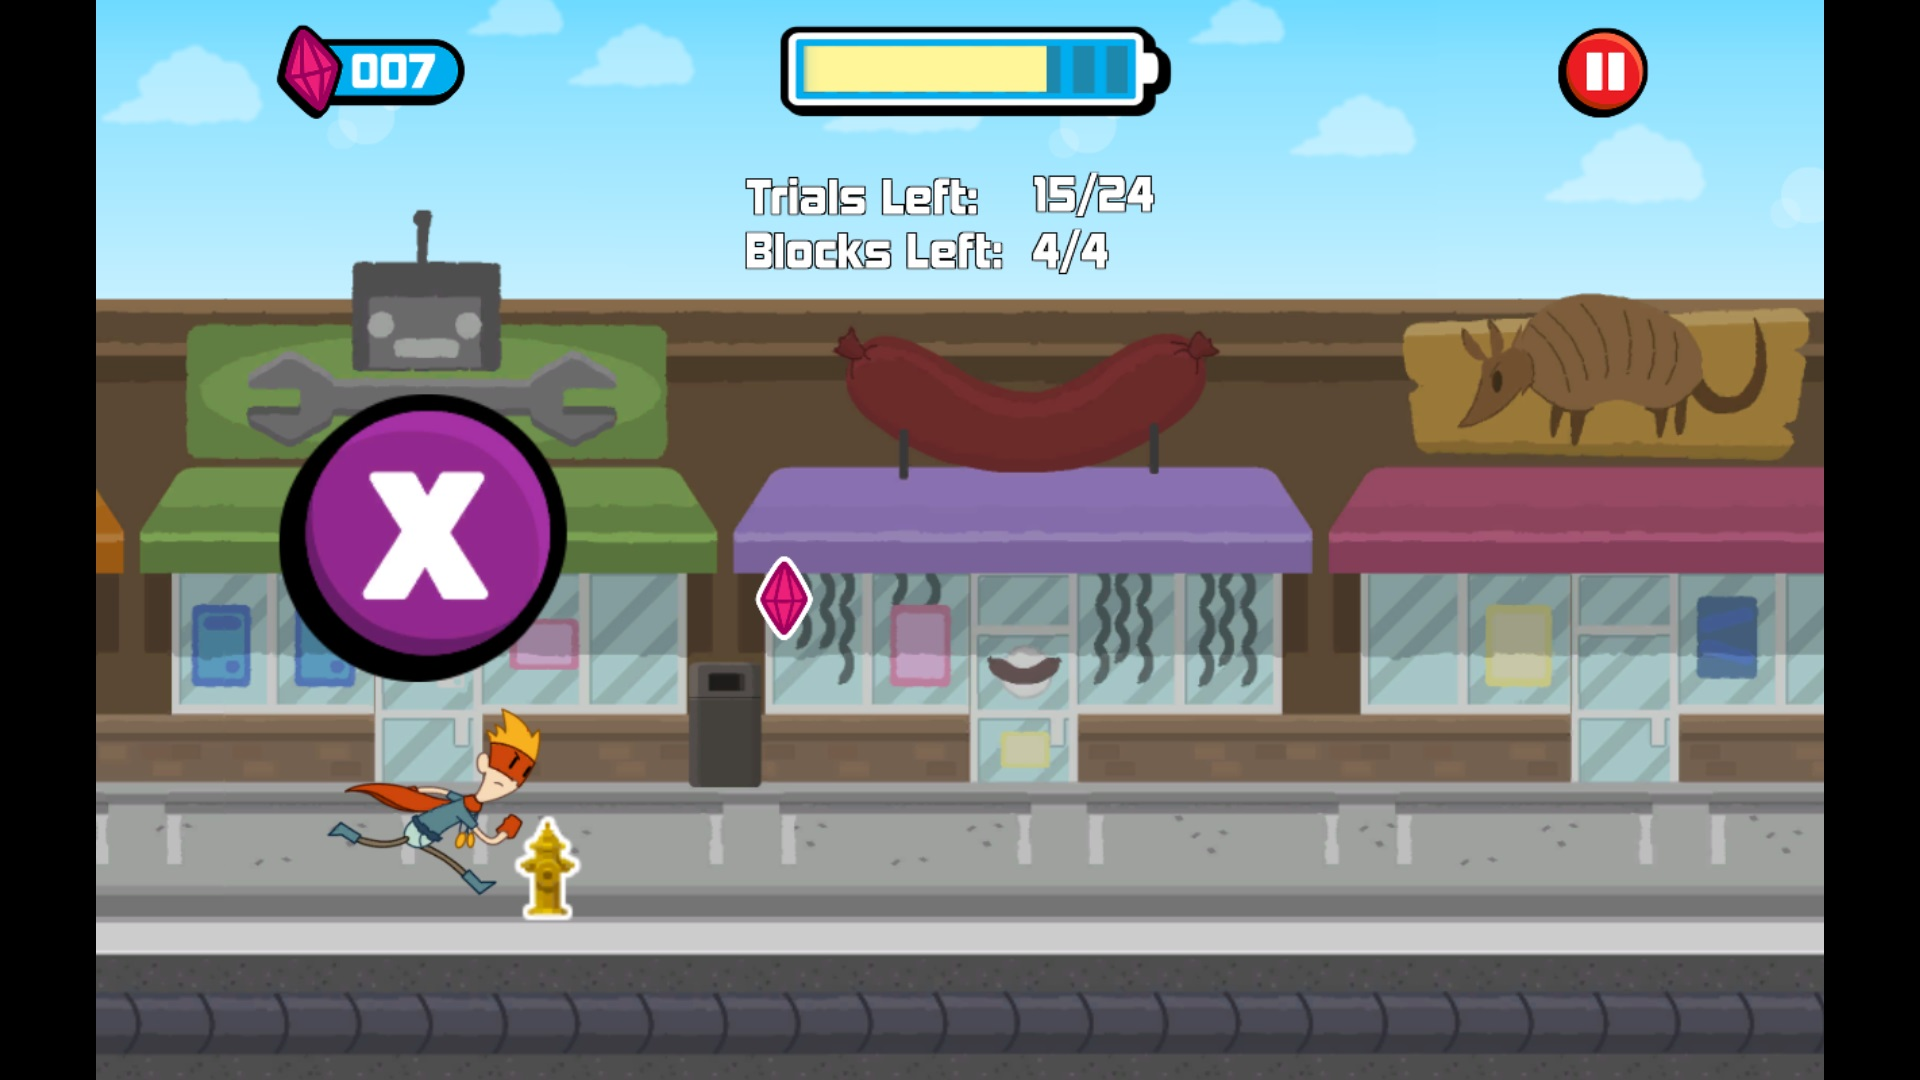
\includegraphics[keepaspectratio]{actiondash.png}}

\end{minipage}%
%
\begin{minipage}{0.50\linewidth}
\subcaption{\label{}Working memory training task}

\pandocbounded{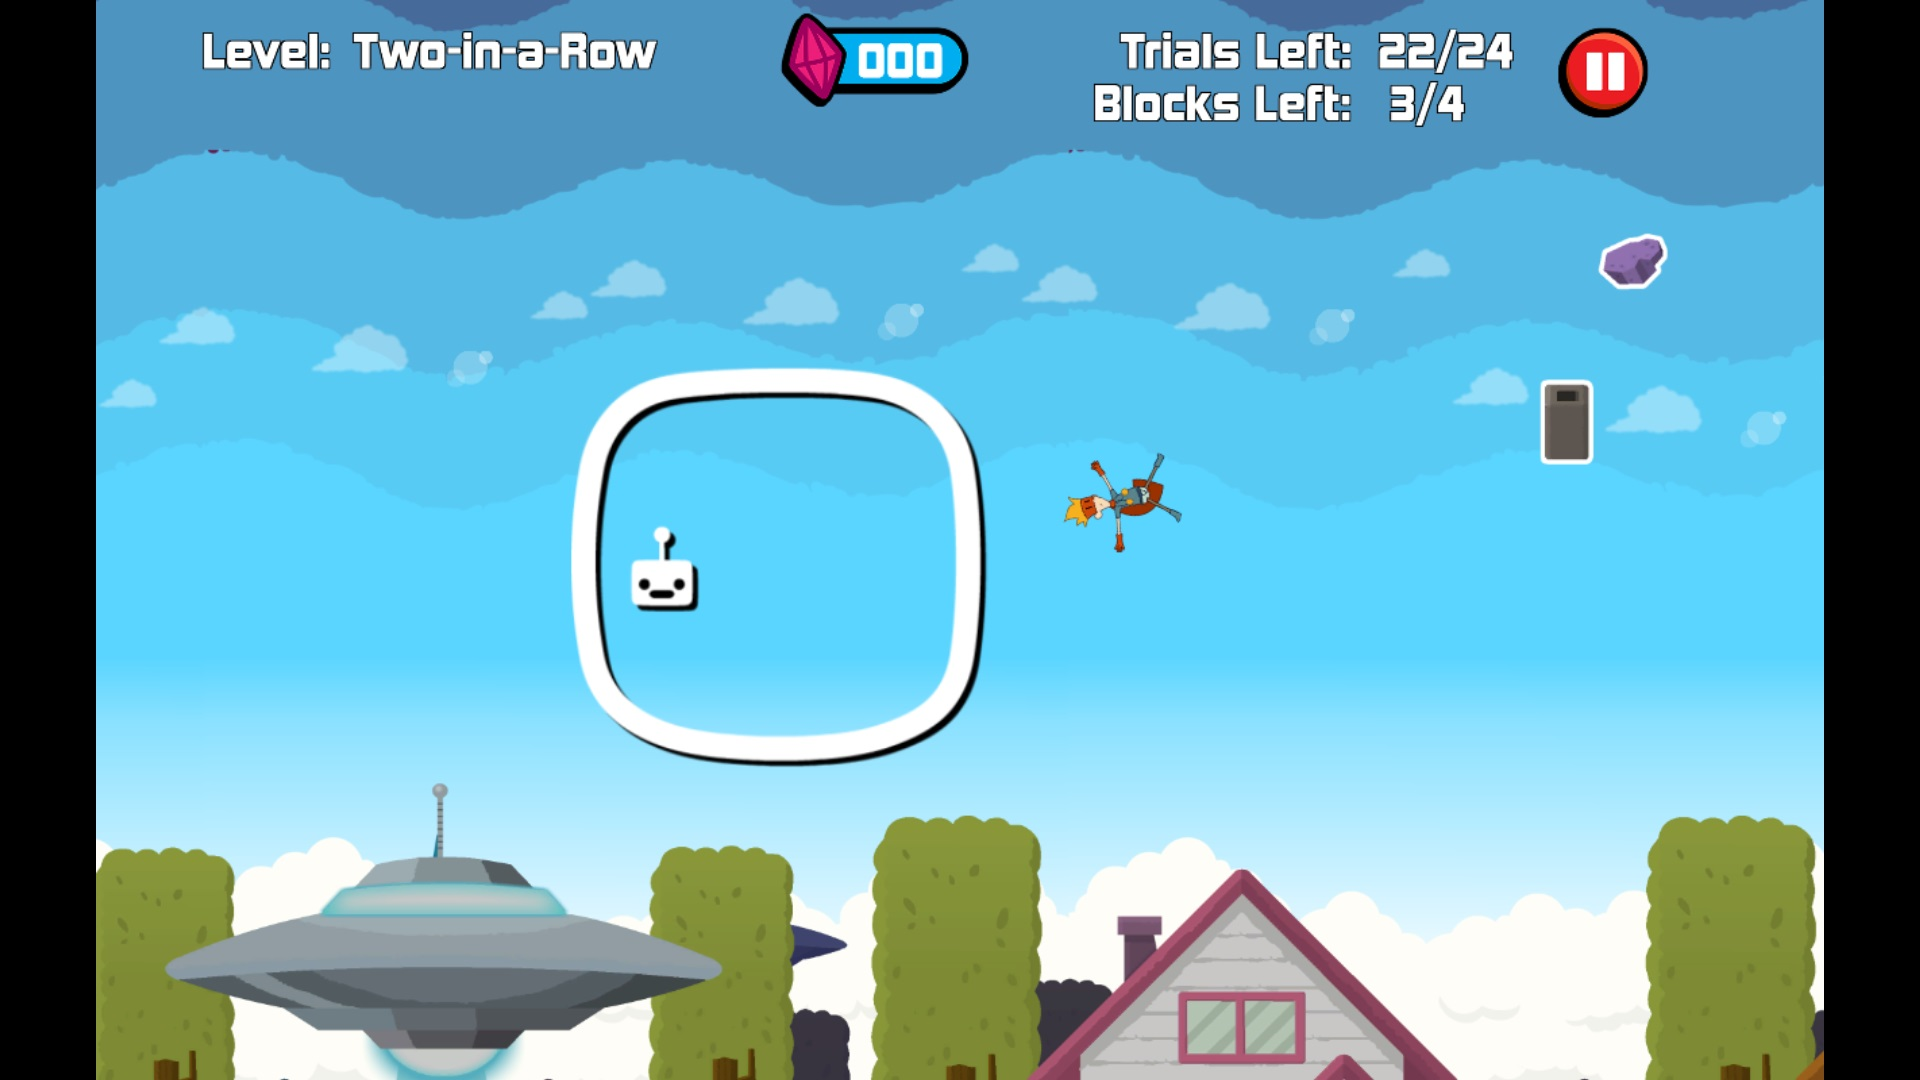
\includegraphics[keepaspectratio]{dangerdive.png}}

\end{minipage}%

\end{figure}%

\section{Analysis}\label{analysis}

Data were screened for validity\ldots{}

\bookmarksetup{startatroot}

\chapter{Results}\label{results}

\section{ADHD Group}\label{adhd-group}

A multiple linear regression model for change in response inhibition
after 5 weeks of intervention with all the predictors (age, gender,
baseline response inhibition, working memory, EF impairment, ADHD
symptoms, autism traits, stimulant medication use, and time on task)
entered revealed a significant model fit indicating that the baseline
characteristics entered predicted response to treatment, accounting for
45\% of the variance (F = 4.7, p \textless{} 0.001, R\textsuperscript{2}
= 0.45). Baseline response inhibition (\(\beta\) = -0.30, p = 0.02) and
baseline working memory (\(\beta\) = -0.40, p = 0.0014) predicted
improvement in response inhibition after 5 weeks regardless of treatment
group such that lower (i.e., worse) baseline response inhibition and
higher (i.e., better) baseline working memory (on the N-Back 1-back
condition) predicted greater improvement after 5 weeks. Additionally,
the model showed a significant interaction effect of baseline response
inhibition by randomization group moderating change in response
inhibition at 5 weeks post-treatment (\(\beta\) = -0.65, p = 0.01),
ruling out the potential for regression to the mean explaining the
result.

This result showed that lower (i.e., worse) baseline response inhibition
was associated with a larger improvement in the Mega Team treatment
group than in the TAU control group in response inhibition after 5 weeks
of treatment. No other factors were significant predictors or moderators
of change in response inhibition after 5 weeks of treatment (see
Table~\ref{tbl-beta1}).

\begin{landscape}

\begin{table}

\caption{\label{tbl-beta1}Multiple Linear Regression Model Results
Predicting Response Inhibition and Working Memory in ADHD group}

\centering{

\centering
\begin{threeparttable}
\resizebox{\ifdim\width>\linewidth\linewidth\else\width\fi}{!}{
\begin{tabular}{lcccccccccccc}
\toprule
\multicolumn{1}{c}{Predictors} & \multicolumn{12}{c}{Outcomes} \\
\cmidrule(l{3pt}r{3pt}){1-1} \cmidrule(l{3pt}r{3pt}){2-13}
\multicolumn{1}{c}{ } & \multicolumn{2}{c}{\makecell[c]{\textbf{Δ SSRT 5 Week} \\F = 4.7* \\R² = 0.45}} & \multicolumn{2}{c}{\makecell[c]{\textbf{Δ SSRT 6 Month} \\F = 6.7* \\R² = 0.55}} & \multicolumn{2}{c}{\makecell[c]{\textbf{Δ 1-back 5 Week} \\F = 2.9* \\R² = 0.32}} & \multicolumn{2}{c}{\makecell[c]{\textbf{Δ 1-back 6 Month} \\F = 2 \\R² = 0.25}} & \multicolumn{2}{c}{\makecell[c]{\textbf{Δ 2-back 5 Week} \\F = 3.2* \\R² = 0.35}} & \multicolumn{2}{c}{\makecell[c]{\textbf{Δ 2-back 6 Month} \\F = 3.5* \\R² = 0.38}} \\
\cmidrule(l{3pt}r{3pt}){2-3} \cmidrule(l{3pt}r{3pt}){4-5} \cmidrule(l{3pt}r{3pt}){6-7} \cmidrule(l{3pt}r{3pt}){8-9} \cmidrule(l{3pt}r{3pt}){10-11} \cmidrule(l{3pt}r{3pt}){12-13}
 & $\beta$ & \textit{p} & $\beta$ & \textit{p} & $\beta$ & \textit{p} & $\beta$ & \textit{p} & $\beta$ & \textit{p} & $\beta$ & \textit{p}\\
\midrule
Stimulants & 0.14 & 0.5 & -0.18 & 0.4 & 0.23 & 0.3 & -0.04 & 0.9 & -0.29 & 0.2 & 0.18 & 0.4\\
Treatment Group & 0.15 & 0.3 & -0.15 & 0.9 & -1.0 & 0.066 & -0.12 & 0.4 & -0.93 & 0.4 & -0.25 & 0.4\\
SNAP Total & 0.16 & 0.2 & 0.19 & 0.11 & -0.03 & 0.8 & 0.11 & 0.5 & 0.03 & 0.8 & 0.10 & 0.5\\
SCQ Score & 0.13 & 0.2 & 0.10 & 0.3 & -0.03 & 0.8 & -0.02 & >0.9 & -0.12 & 0.3 & -0.21 & 0.071\\
SSRT & -0.30 & \textbf{0.022} & -0.65 & \textbf{<0.001} & -0.12 & 0.4 & -0.17 & 0.3 & -0.17 & 0.2 & -0.20 & 0.12\\
Target Accuracy (1-back) & -0.40 & \textbf{0.001} & -0.38 & \textbf{0.001} & -0.56 & \textbf{<0.001} & -0.59 & \textbf{<0.001} & 0.15 & 0.2 & 0.05 & 0.7\\
Target Accuracy (2-back) & 0.06 & 0.6 & -0.02 & 0.9 & 0.15 & 0.3 & 0.02 & 0.9 & -0.43 & \textbf{0.003} & -0.55 & \textbf{<0.001}\\
BRIEF-2 GEC & -0.11 & 0.5 & -0.12 & 0.4 & 0.01 & >0.9 & -0.23 & 0.2 & -0.08 & 0.6 & -0.10 & 0.5\\
Age & 0.21 & 0.066 & -0.04 & 0.7 & -0.08 & 0.5 & 0.29 & \textbf{0.034} & 0.22 & 0.063 & 0.19 & 0.12\\
Gender & 0.02 & >0.9 & 0.59 & \textbf{0.011} & 0.31 & 0.2 & -0.14 & 0.6 & -0.09 & 0.7 & 0.10 & 0.7\\
Time on task & -0.15 & 0.5 & -0.05 & 0.8 & 0.46 & \textbf{0.037} & 0.02 & >0.9 & 0.17 & 0.5 & 0.07 & 0.7\\
Stimulants * Treatment Group & -0.16 & 0.6 & 0.43 & 0.11 & -0.10 & 0.7 & 0.17 & 0.6 & 0.45 & 0.2 & -0.04 & >0.9\\
Treatment Group * SNAP Total & 0.05 & 0.8 & 0.01 & >0.9 & -0.20 & 0.4 & 0.01 & >0.9 & 0.09 & 0.7 & 0.25 & 0.3\\
Treatment Group * SCQ Score & -0.24 & 0.14 & -0.13 & 0.4 & -0.11 & 0.5 & -0.12 & 0.5 & -0.02 & >0.9 & 0.01 & >0.9\\
Treatment Group * SSRT & -0.43 & \textbf{0.010} & -0.19 & 0.2 & 0.10 & 0.6 & 0.09 & 0.7 & 0.24 & 0.2 & 0.00 & >0.9\\
Treatment Group * Target Accuracy (1-back) & 0.22 & 0.2 & 0.43 & \textbf{0.013} & 0.10 & 0.6 & 0.23 & 0.3 & 0.27 & 0.2 & 0.61 & \textbf{0.002}\\
Treatment Group * Target Accuracy (2-back) & -0.06 & 0.7 & -0.14 & 0.4 & -0.06 & 0.8 & -0.10 & 0.6 & -0.27 & 0.15 & -0.19 & 0.3\\
Treatment Group * BRIEF-2 GEC & -0.06 & 0.8 & -0.06 & 0.8 & 0.10 & 0.7 & 0.26 & 0.3 & -0.15 & 0.5 & -0.13 & 0.6\\
Treatment Group * Age & -0.11 & 0.5 & -0.03 & 0.9 & 0.33 & 0.076 & -0.19 & 0.3 & 0.05 & 0.8 & -0.07 & 0.7\\
Treatment Group * Gender & 0.04 & 0.9 & -0.53 & 0.11 & -0.54 & 0.13 & 0.00 & >0.9 & -0.03 & >0.9 & -0.21 & 0.6\\
\bottomrule
\end{tabular}}
\begin{tablenotes}[para]
\item \textit{Note: } 
\item SSRT - Stop Signal Reaction Time. *\textit{p}-value < 0.0035 (Bonferroni corrected); Bold p-value < 0.05.
\end{tablenotes}
\end{threeparttable}

}

\end{table}%

\end{landscape}

\section{Autism Group}\label{autism-group}

In the autism group\ldots.

\bookmarksetup{startatroot}

\chapter{Discussion}\label{discussion}

\section{Main Findings}\label{main-findings}

This project aimed to explore the impact of\ldots{}

\subsection{ADHD Group}\label{adhd-group-1}

In the current study\ldots{}

\subsection{Autism Group}\label{autism-group-1}

Results showed\ldots{}

\section{Strengths \& Limitations}\label{strengths-limitations}

Strengths of this study include\ldots{}

\section{Implications \& Future
Directions}\label{implications-future-directions}

Future research directions\ldots{}

\bookmarksetup{startatroot}

\chapter*{References}\label{references}
\addcontentsline{toc}{chapter}{References}

\markboth{References}{References}

\phantomsection\label{refs}
\begin{CSLReferences}{1}{0}
\bibitem[\citeproctext]{ref-americanpsychiatricassociation2022}
American Psychiatric Association. (2022). \emph{Diagnostic and
statistical manual of mental disorders : {DSM-5-TR}} (5th edition, text
revision.). American Psychiatric Association Publishing.
\url{https://doi/book/10.1176/appi.books.9780890425787}

\bibitem[\citeproctext]{ref-ayano2023}
Ayano, G., Demelash, S., Gizachew, Y., Tsegay, L., \& Alati, R. (2023).
The global prevalence of attention deficit hyperactivity disorder in
children and adolescents: {An} umbrella review of meta-analyses.
\emph{Journal of Affective Disorders}, \emph{339}, 860--866.
\url{https://doi.org/10.1016/j.jad.2023.07.071}

\bibitem[\citeproctext]{ref-bussing2008}
Bussing, R., Fernandez, M., Harwood, M., Hou, W., Garvan, C. W.,
Swanson, J. M., \& Eyberg, S. M. (2008). Parent and teacher {SNAP-IV}
ratings of attention deficit/hyperactivity disorder symptoms:
{Psychometric} properties and normative ratings from a school district
sample. \emph{Assessment}, \emph{15}(3), 317--328.
\url{https://doi.org/10.1177/1073191107313888}

\bibitem[\citeproctext]{ref-cheungRCT}
Cheung, T. C. K., Ram, N., Anagnostou, E., Ameis, S. H., Sananes, R.,
Bedard, A.-C., \& Crosbie, J. (in prep). \emph{Cognitive rehabilitation
({Mega Team}) and its effects on emotional and behavioural regulation in
{ADHD} and {ASD} children}.

\bibitem[\citeproctext]{ref-faraone2021}
Faraone, S. V., Banaschewski, T., Coghill, D., Zheng, Y., Biederman, J.,
Bellgrove, M. A., Newcorn, J. H., Gignac, M., Al Saud, N. M., Manor, I.,
Rohde, L. A., Yang, L., Cortese, S., Almagor, D., Stein, M. A., Albatti,
T. H., Aljoudi, H. F., Alqahtani, M. M. J., Asherson, P., \ldots{} Wang,
Y. (2021). The world federation of {ADHD} international consensus
statement: 208 evidence-based conclusions about the disorder.
\emph{Neuroscience \& Biobehavioral Reviews}, \emph{128}, 789--818.
\url{https://doi.org/10.1016/j.neubiorev.2021.01.022}

\bibitem[\citeproctext]{ref-french2024}
French, B., Nalbant, G., Wright, H., Sayal, K., Daley, D., Groom, M. J.,
Cassidy, S., \& Hall, C. L. (2024). The impacts associated with having
{ADHD}: An umbrella review. \emph{Frontiers in Psychiatry}, \emph{15}.
\url{https://doi.org/10.3389/fpsyt.2024.1343314}

\bibitem[\citeproctext]{ref-ickowicz2006}
Ickowicz, A., Schachar, R. J., Sugarman, R., Chen, S. X., Millette, C.,
\& Cook, L. (2006). The parent interview for child symptoms: A
situation-specific clinical research interview for attention-deficit
hyperactivity and related disorders. \emph{Canadian Journal of
Psychiatry.}, \emph{51}(5), 325--328.
\url{https://doi.org/10.1177/070674370605100508}

\bibitem[\citeproctext]{ref-logan1997}
Logan, G. D., Schachar, R. J., \& Tannock, R. (1997). Impulsivity and
inhibitory control. \emph{Psychological Science}, \emph{8}(1), 60--64.
\url{https://doi.org/10.1111/j.1467-9280.1997.tb00545.x}

\bibitem[\citeproctext]{ref-lord2012}
Lord, C., Rutter, M., DiLavore, P., Risi, S., Gotham, K., \& Bishop, S.
(2012). \emph{Diagnostic observation schedule, second edition ({ADOS-2})
manual (part {I}): {Modules} 1-4}. Western Psychological Services.

\bibitem[\citeproctext]{ref-pettersson2019}
Pettersson, E., Lichtenstein, P., Larsson, H., Song, J., Agrawal, A.,
Børglum, A. D., Bulik, C. M., Daly, M. J., Davis, L. K., Demontis, D.,
Edenberg, H. J., Grove, J., Gelernter, J., Neale, B. M., Pardiñas, A.
F., Stahl, E., Walters, J. T. R., Walters, R., Sullivan, P. F., \ldots{}
Polderman, T. J. C. (2019). Genetic influences on eight psychiatric
disorders based on family data of 4 408 646 full and half-siblings, and
genetic data of 333 748 cases and controls. \emph{Psychological
Medicine}, \emph{49}(7), 1166--1173.
\url{https://doi.org/10.1017/S0033291718002039}

\bibitem[\citeproctext]{ref-posar2019}
Posar, A., \& Visconti, P. (2019). Long-term outcome of autism spectrum
disorder. \emph{Turkish Archives of Pediatrics/Türk Pediatri Arşivi},
\emph{54}(4), 207--212.
\url{https://doi.org/10.14744/TurkPediatriArs.2019.16768}

\bibitem[\citeproctext]{ref-swanson1981}
Swanson, J. M., Nolan, W., \& Pelham, W. (1981). \emph{Paper presented
at the meeting of the american psychological association}.

\end{CSLReferences}

\cleardoublepage
\phantomsection
\addcontentsline{toc}{part}{Appendices}
\appendix

\chapter{Questionnaire}\label{sec-apx1}

\appendices{A Questionnaire}

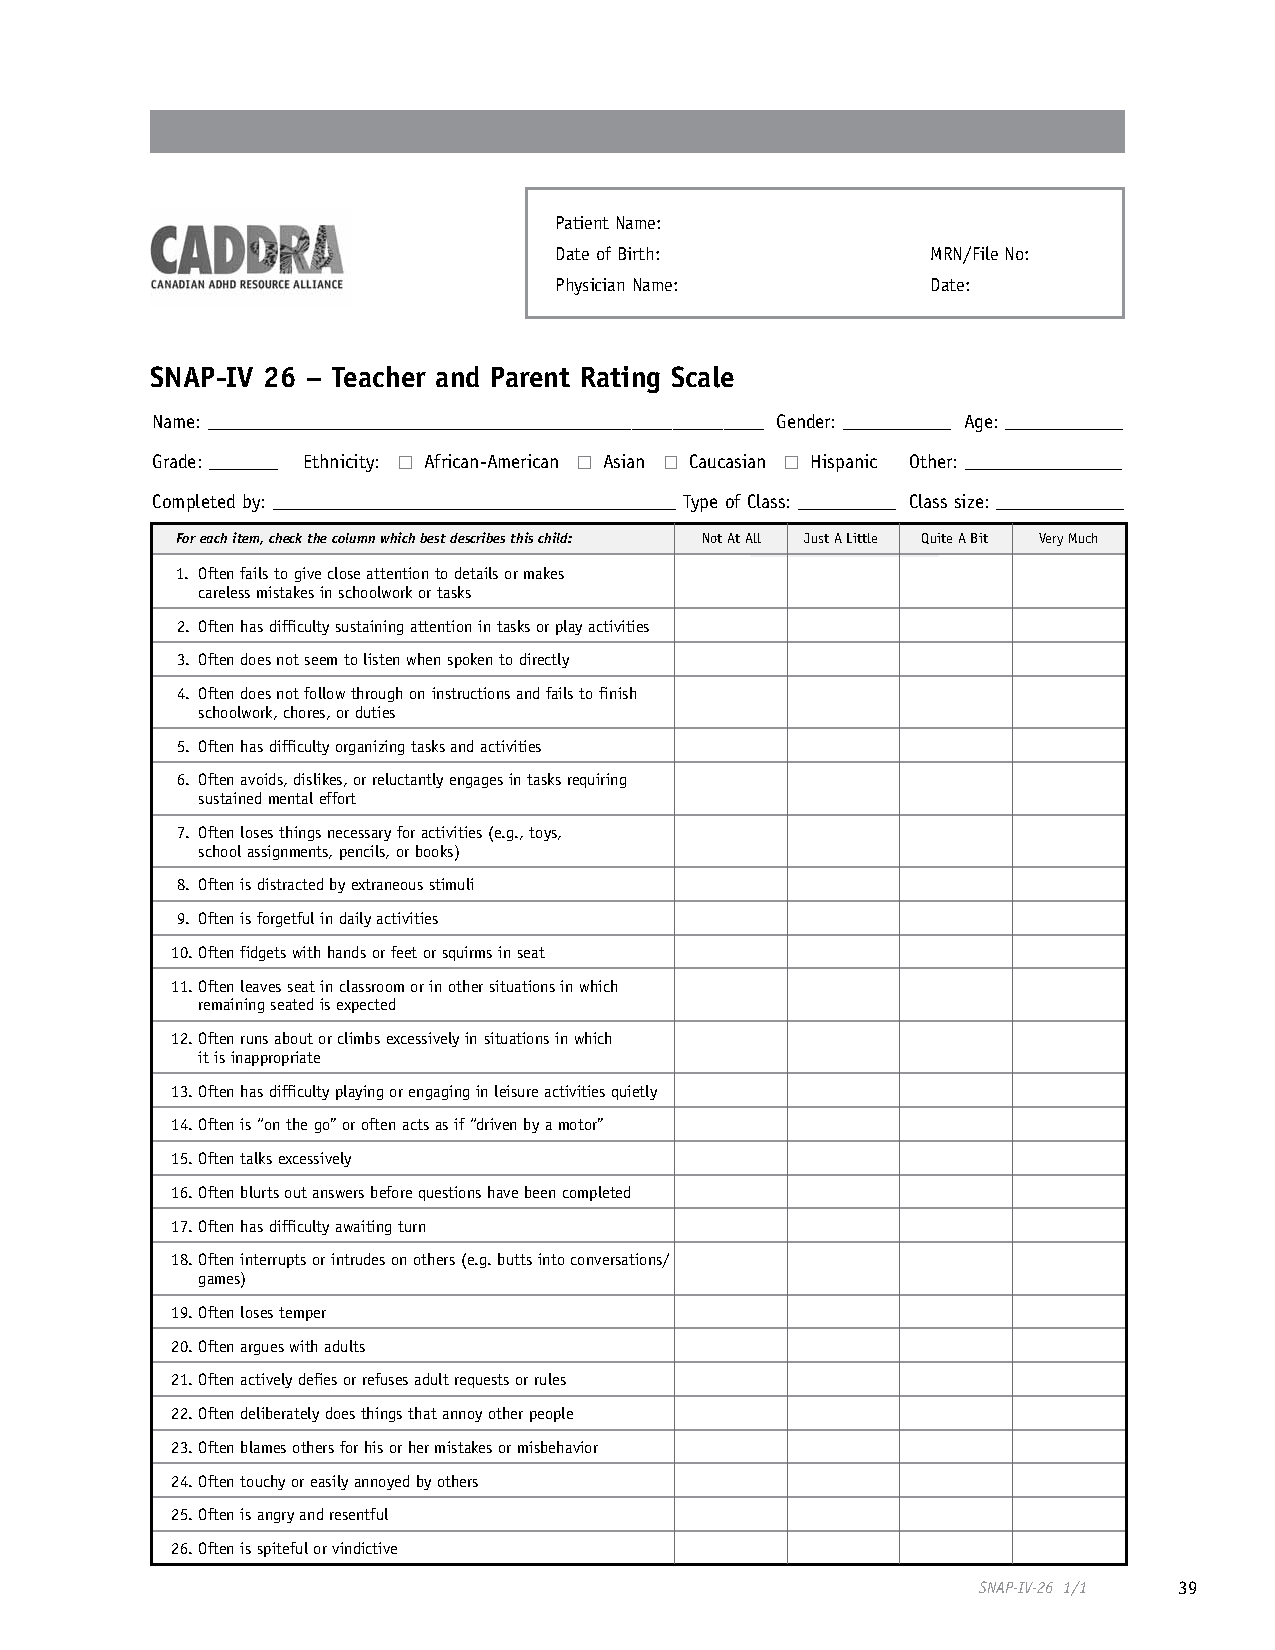
\includepdf[pages=1, pagecommand={}, scale = 0.85]{apx1-snap.pdf}




\end{document}
